\input{../std.tex}

\begin{document}
  \begin{center}
    \LARGE \textbf{Física Computacional} \\
    \Large \textbf{Tarefa 7 - Questão 4} \\
    \large Alex Enrique Crispim
  \end{center}

  Considere o problema de valor inicial (PVI) abaixo
  \begin{equation*}
    x^{\prime \prime} = a(t, x), \\
    x(0) = x_0 \qc x^\prime(0) = v_0.
  \end{equation*}

  Denotemos $x^\prime$ por $v$. O método de Euler-Cromer para EDOs de ordem 2 consiste em utilizar as mesmas expressões para o método de Euler, porém atualizando as derivadas $v$ primeiro.
  De forma mais explicita, ao invés de utilizarmos as equações
  \begin{flalign*}
    x_{i+1} = x_i + h v_i \qc
    v_{i+1} = v_i + h a_i,
  \end{flalign*}
  nessa ordem, utilizamos
  \begin{flalign*}
    v_{i+1} = v_i + h a_i, \\ 
    x_{i+1} = x_i + h v_{i+1}.
  \end{flalign*}

  De forma mais geral, poderiamos ter $\dv{x}{t} = f(t, v)$ e $\dv{v}{t} = g(t, x)$. Calculariamos primeiramente $v_{i+1}$ e então $x_{i+1}$ como $x_{i+1} = x_i + h g(t_i, v_{i+1})$.

  Um modo de se fazer isso para o sistema abaixo
  \begin{equation}
    \begin{cases}
      \dt{\omega} = -(g/L) sin(\theta) - q \omega + F_d \sin(\omega_d t), \\
      \dt{\theta} = \omega,
    \end{cases}
    \label{eq:1}
  \end{equation}
  é calcular $\omega$ primeiramente e utilizar seu valor diretamente no calculo de $\theta$, sem precisar de uma nova variável para guardar o antigo valor de $\omega$. Isso poupa espaço e processamento. Uma implementação utilizando tal ideia foi feita na pasta \textit{question 4} em \url{https://github.com/AlexEnrique/comp-physics-pratice7}.
  \begin{figure}[h]
    \center
    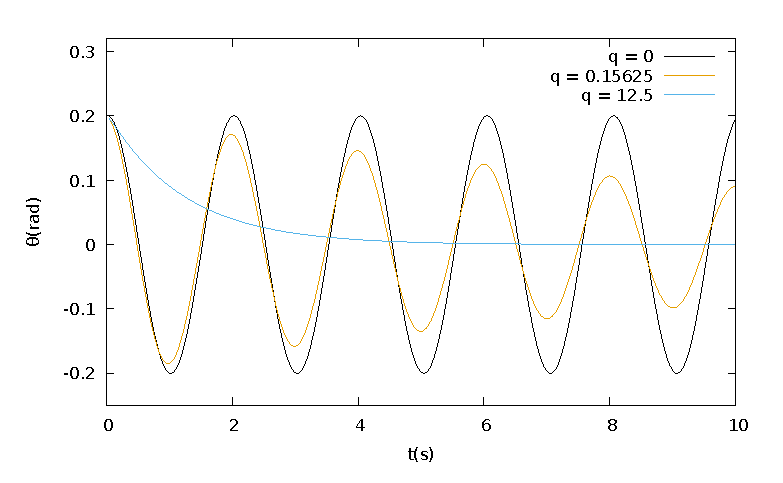
\includegraphics[scale = .5]{q4Figs}
    \caption{Gráfico das soluções de (\ref{eq:1}) variando-se o valor de $q$}
  \end{figure}





\end{document}
